
\begin{chapter}{Validation and Benchmarking\label{chap:valid}}
  
  For all new computer programs, an important step in the development
  process is the program's validation against other computational
  tools.  In the field of fusion activation calculations, there are
  many such tools.  Both FISPACT-97\cite{FISPACT} (time-step based ODE
  solver) and DKR\cite{DKR} (no-loop Bateman solution to linear
  chains) have been shown in the past to agree well with analytical
  solutions to multi-step activation
  pathways\cite{IAEA.bench2.rep,ITER.exp.valid}.  \ALARA\ offers
  improvement over DKR because it is able to accurately model loops in
  the activation trees and calculate the gas production.  In
  comparison to FISPACT-97, \ALARA\ has many advantages, including the
  ability to exactly model pulsed irradiation histories and
  simultaneously calculate the solution at many spatial points.  In
  comparison to both codes, \ALARA\ uses modern programming practices
  and data handling to increase the flexibility of operation and
  reduce memory requirements (see section \ref{sec:summary.modern}).

  \begin{section}{Benchmark Specifications}
  
    To validate \ALARA\ the International Atomic Energy Agency [IAEA]
    Fusion Evaluated Nuclear Data Library [FENDL] Calculational
    Activation Benchmark\cite{IAEA.bench1.spec} problem was chosen.
    This problem is based on the reference steel/water shielding
    blanket design in the International Thermonuclear Experimental
    Reactor [ITER] outline design.  This design includes:
    \begin{itemize}
    \item a copper first wall with beryllium coating
    \item shielding blanket with alternating layers of stainless steel
      (316 SS) and water
    \item a double wall Inconel 625 vacuum vessel with a water-cooled
      steel pebble bed and a back shield made of lead and boron carbide
    \item an inboard magnet, including conductors and insulators.
    \end{itemize}
    With such a wide range of materials, the design offers an
    extensive test of the activation code's capabilities.
    
    The neutron fluxes have been provided by the benchmark in the
    VITAMIN-J 175 group energy structure for each of the 468 fine mesh
    intervals.  These fluxes were calculated using the
    ONEDANT\cite{ONEDANT} deterministic neutron transport code with a
    14.1 MeV isotropic neutron source normalized to inboard and
    outboard neutron wall loadings of 1 and 1.5 MW/m$^2$,
    respectively.
    
    IAEA Fusion Evaluated Nuclear Data Library (ver. 2.0) for
    Activation (FENDL/A 2.0) and for Decay (FENDL/D 2.0) were used for
    all calculations, ensuring that difference in the results were due
    to the activation codes themselves and not the nuclear data.
    
    The first activation calculations were performed with a steady
    state operation time of 3 years and cooling times of 1 hour, 1
    day, 1 week, 30 days, 1 year and 100 years.  A pulsed activation
    calculation was also performed using 94500 pulses of 1000 s with a
    dwell time of 1200 s between pulses.
  \end{section}
  
  \begin{section}{Steady-State Problem}
    
    In \ALARA\, this calculation built 109 reaction trees with a total
    of 32023 nodes and a longest chain of length 14, producing 603
    different isotopes in the steel-containing intervals, of which 402
    were radioactive.  The truncation tolerance was $10^{-4}$ and the
    ignore tolerance, $10^{-6}$.
    
    The results have been compared by calculating the relative
    difference between \ALARA\ and the other codes:
    $$\mbox{Relative Difference} = \frac{\mbox{\ALARA}}{\mbox{X}} - 1,$$
    where X is either FISPACT-97 or DKR.  
    
    \begin{figure}[htbp]
      \begin{center}
        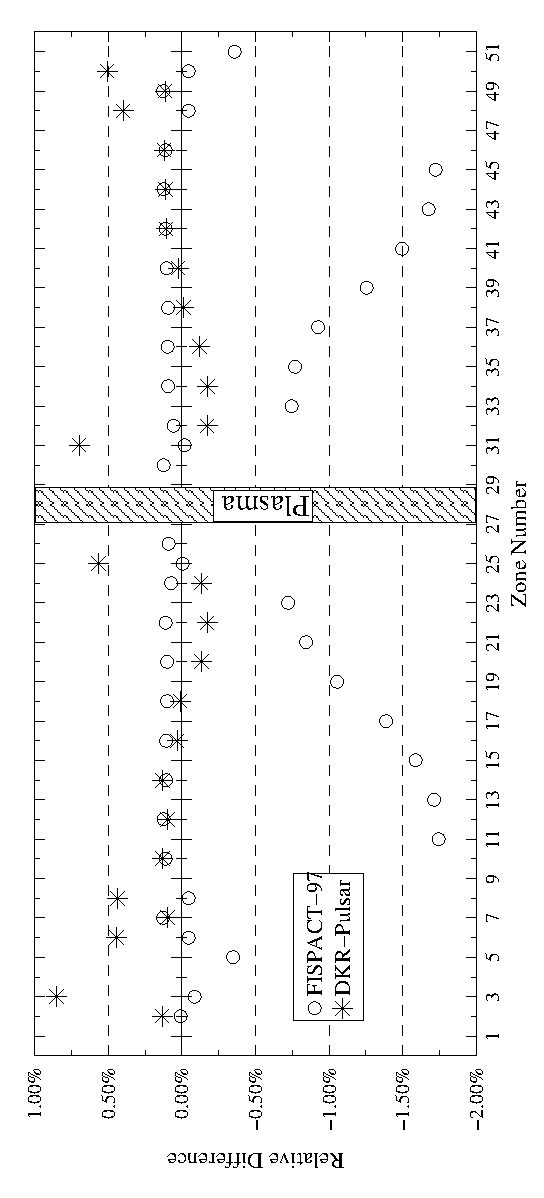
\epsfig{file=eps/1h_final.eps,height=\textwidth,angle=-90}
        \caption{Relative difference between ALARA and other codes for
          steady state problem at a cooling time of 1 hour.}
        \label{fig:rel.diff.ss.1}
      \end{center}
    \end{figure}
    
    \begin{figure}[htbp]
      \begin{center}
        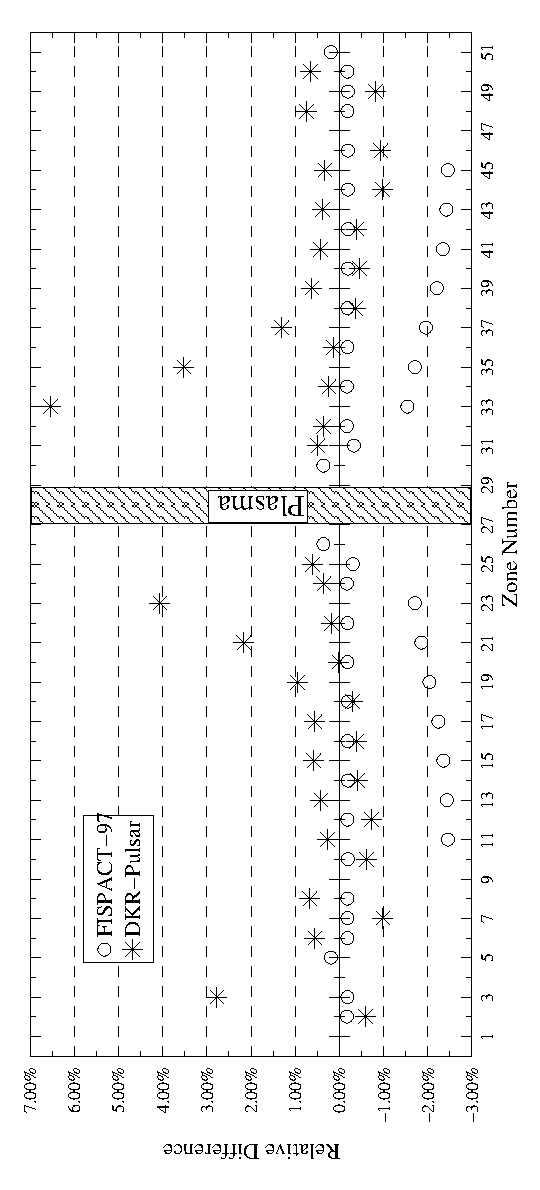
\epsfig{file=eps/1c_final.eps,height=\textwidth,angle=-90}
        \caption{Relative difference between \ALARA\  and other codes for
          steady state problem at a cooling time of 1 century.}
        \label{fig:rel.diff.ss.2}
      \end{center}
    \end{figure}
    
    Figures \ref{fig:rel.diff.ss.1} and \ref{fig:rel.diff.ss.2} show
    the relative difference between the steady state problem's results
    from \ALARA\ and FISPACT-97 and between \ALARA\ and DKR at a
    cooling time of 1 hour and 1 century, respectively.
    
    At a cooling time of 1 hour, the \ALARA\ results are within 1.8\%
    of the FISPACT-97 results throughout the entire geometry, with
    most zones having a difference of less than 0.4\%.  The largest
    differences occur in the blanket's 14 water-filled zones,
    increasing in directions away from the plasma as flux becomes
    lower and softer.
    \enlargethispage*{\baselineskip}
    
    At a cooling time of 1 century, the differences between \ALARA\ 
    and FISPACT-97 are as high as 2.5\%, with the largest differences
    still occurring in the water-filled zones where, after more than 8
    tritium half-lives, the dominant isotope is now $^{14}$C.  The
    differences in the other zones remain below 0.4\%.
    
    The results from these comparisons immediately demonstrate the
    impact of the various activation codes different methods.  In most
    zones, the \ALARA\ results are within a fraction of a percent of
    the FISPACT-97 values.  In the water-filled zones, alternating
    with the steel in the inboard and outboard blanket, the total
    activity was greatly underestimated.  Further investigation shows
    that the activity is dominated by tritium and $^{14}$C, and that
    their relative production levels are as low as $5 \times 10^{-12}$
    and $3 \times 10^{-9}$, respectively.  It is clear that this level
    of accuracy is not sufficient for these zones.  On the other hand,
    increasing the accuracy for the whole problem would dramatically
    increase the activation tree size in all the other zones.  While
    this demonstrates the limitations of a problem-wide truncation
    tolerance, it requires little effort to perform a second \ALARA\ 
    calculation.  A second calculation was performed for this problem
    using $10^{-10}$ for both the truncation and ignore tolerances.
    Figures \ref{fig:rel.diff.ss.1} and \ref{fig:rel.diff.ss.2} are
    based on these values in the odd numbered zones between 11 and 23
    and between 33 and 45, inclusively.
    
    DKR had an even more drastic problem with zones where the specific
    activity was dominated by tritium.  Since the methods implemented
    in this version of DKR were not designed to compute the
    accumulation of light ions ($^1$H, $^2$H, $^3$H, $^3$He, and
    $^4$He) emitted by nuclear reactions, the major source of tritium,
    its total activity for all zones with dominant tritium inventories
    is much too small.  Since these differences were up to a few
    orders of magnitude, the relative difference between \ALARA\ and
    DKR in these zones has not been shown in figure
    \ref{fig:rel.diff.ss.1} in order to compare the differences in the
    other zones.  The magnitude of these differences can be inferred,
    however, from figure \ref{fig:rel.diff.ss.2}, where it must be
    noted that 1 century is over 8 tritium half-lives.  The
    undercalculation of tritium in these zones is so great that even
    after more than 99.6\% of the tritium has decayed, the error is
    still a few percent.
    
    In those zones with insignificant tritium inventories, the
    differences between \ALARA\ and DKR are less than 0.2\% throughout
    the geometry at a cooling time of 1 hour.  After 1 century, even
    though the relative contribution of tritium has increased in some
    of those same zones, the relative differences are still less than
    1\%.  DKR's inability to account for the light ion production
    results in tritium inventories as much as 6 orders of magnitude
    too low in the first wall's Be coating, and up to 3 times too low
    in the blanket's water cooled zones.  Even after more than 8
    tritium half-lives (1 century), when tritium is responsible for
    less than 10\% of the total activity, the difference between
    \ALARA\ and DKR in the water can be as high as 7\% (zone \#33).
    This discrepancy demonstrates why the modeling of light ion
    accumulation is a base features for any new activation code.
    
    A single fine mesh interval was chosen in which to compare the
    activity of various nuclides in detail.  The 1 mm thick stainless
    steel (SS316) inboard first wall back plate is modeled as a single
    interval (\#242) in zone \#24.  The large number of initial
    isotopes in steel and the high flux due to its proximity to the
    plasma make this a good choice for comparison.
    
    Table \ref{tab:detail.1} shows the seven most dominant isotopes at
    a cooling time of 1 hour, together accounting for over 95\% of the
    total activity.  Table \ref{tab:detail.2} shows the five most
    dominant isotopes at a cooling time of 1 century, accounting for
    more than 99.7\% of the total activity.

    \begin{table}[htbp]
      \begin{center}
        \caption{Detailed differences in interval \#242 at 1 hour.}
        \label{tab:detail.1}
        \begin{tabular}{|c|c|c|c|}
          \hline
          Isotope & \ALARA\  & \multicolumn{2}{c|}{Relative Difference [\%]} \\
          & [10$^{16}$Bq/m$^3$] & FISPACT-97 & DKR-Pulsar 2.0\\\hline
          $^{56}$Mn & 114.6 & -0.051 & 0.15 \\\hline
          $^{55}$Fe & 85.5 & 0.24 & -0.10 \\\hline
          $^{51}$Cr & 75.7 & 0.019 & -0.041 \\\hline
          $^{57}$Co & 24.4 & -0.081 &  3.0  \\\hline
          $^{54}$Mn & 20.0 & 0.97  &  0.15 \\\hline
          $^{58m}$Co & 10.3 & -0.053 & 0.30 \\\hline
          $^{58}$Co & 8.32 & -0.048 & -13.74  \\\hline
        \end{tabular}
      \end{center}
    \end{table}
    
    \begin{table}[htbp]
      \begin{center}
        \caption{Detailed differences in interval \#242 at 1 century.}
        \label{tab:detail.2}
        \begin{tabular}{|c|c|c|c|}
          \hline
          Isotope & \ALARA\  & \multicolumn{2}{c|}{Relative Difference [\%]} \\
          & [10$^{13}$Bq/m$^3$] & FISPACT-97 & DKR-Pulsar 2.0\\\hline
          $^{63}$Ni & 27.8 & -0.17 &  0.40 \\\hline
          $^{59}$Ni & 3.80 & -0.18  & -1.2 \\\hline
          $^{91}$Nb & 3.37 & -0.21  &  1.3  \\\hline
          $^{14}$C  & 0.86 & -0.22  & -0.19 \\\hline
          $^{93}$Mo & 0.69 & -0.21  & 16   \\\hline
        \end{tabular}
      \end{center}
    \end{table}
    
    The agreement between \ALARA\ and FISPACT-97 is seen to be within
    1\% in all cases.  DKR, on the other hand, has relative
    differences of up to 16\%.  These discrepancies are most probably
    caused by the inability of DKR to model certain kinds of loops in
    the decay chains and the influence this has on the decay chain
    creation calculations.
    
  \end{section}

  \begin{section}{Pulsing Problem\label{sec:valid.pulse}}
    
    The results of \ALARA\ and DKR for the pulsing problem are
    compared in Figure \ref{fig:rel.diff.p.1} for both 1 hour and 1
    century.  There are no results for FISPACT-97 as it was unable to
    solve the exact pulsing problem in a reasonable amount of time.
    Based on the time (14 minutes) required to solve the first 100
    pulses at a single spatial point, FISPACT-97 was determined to be
    unsuited to such pulsed operation calculations.  Assuming that the
    total computation time scales linearly with the number of pulses,
    the full problem would require more than 220 days for each of the
    317 spatial points -- a total computation time of over 190 years!
    
    Once again, tritium plays an important role in the discrepancies
    which are nearly identical to the discrepancies between \ALARA\ 
    and DKR for the steady state problem.  In TF coil's glass
    insulator (zone \#3), the discrepancy in the pulsing problem is
    twice as high as in the steady state problem at 1 hour, but the
    same at 1 century.  This demonstrates the true physical effect of
    pulsing on the tritium inventory's importance at relatively short
    cooling times, even though the tritium inventory itself is not
    significantly affected by the pulsed history.
    
    The pulsed operation will tend to reduce the inventory of isotopes
    with half-lives of the same order of magnitude as the dwell time
    between pulses: very long-lived isotopes will decay little between
    pulses and slowly reach their saturation level while very
    short-lived isotopes will decay completely between pulses, but can
    reach their saturation level in a single pulse\cite{Pulsar}.  The
    dominant isotopes in the glass at 1 hour are $^{64}$Cu and
    $^{24}$Na, both with half-lives slightly longer than half a day.
    Their inventories in the pulsed problem are 50\% less than in the
    steady state problem, while the tritium inventory is reduced by
    less than 10\%.  Thus, the fraction of the total activity from
    tritium is increased, even though the tritium inventory itself
    goes down.

    \begin{figure}[htbp]
      \begin{center}
        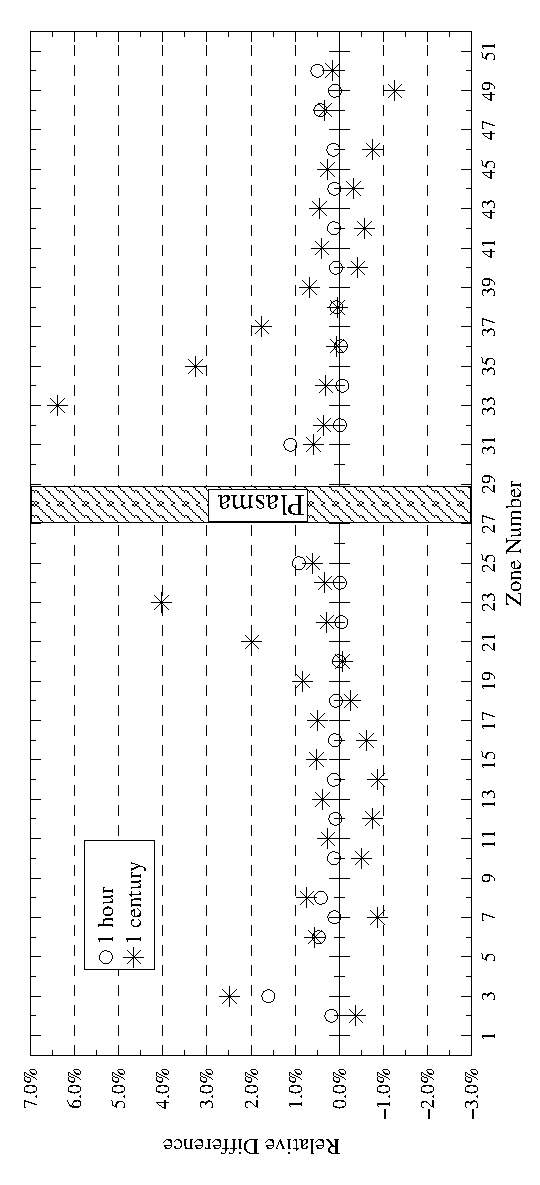
\epsfig{file=eps/pulse_final.eps,height=\textwidth,angle=-90}
        \caption{Relative difference between \ALARA\  and DKR for
          the pulsing problem at cooling times of 1 hour and 1 century.}
        \label{fig:rel.diff.p.1}
      \end{center}
    \end{figure}
    
    One method of modeling a pulsed problem as a steady state problem
    is to preserve both the total fluence and the total operating
    time\cite{Pulsar,hosny,qingming}.  Using ALARA, the results of
    such an approximate calculation with a flux scaling factor of
    1/2.2 and total operation time of 2.079 $\times$ 10$^8$ are
    compared to the exact solution in Figure
    \ref{fig:rel.diff.approx}, represented as
    $$\mbox{Relative Difference} = \frac{\mbox{Pulsing}}{\mbox{Steady
        State}} - 1.$$
    In this case, due to the nature of the pulsing
    history, the effect can only be seen at short cooling times.  As
    discussed above, the pulses' effect is greatest for isotopes with
    half-lives of roughly the same order of magnitude as the dwell
    time between pulses.  Thus the effect decays away within a few
    ``dwell times'' of shutdown.
    
    \begin{figure}[htbp]
      \begin{center}
        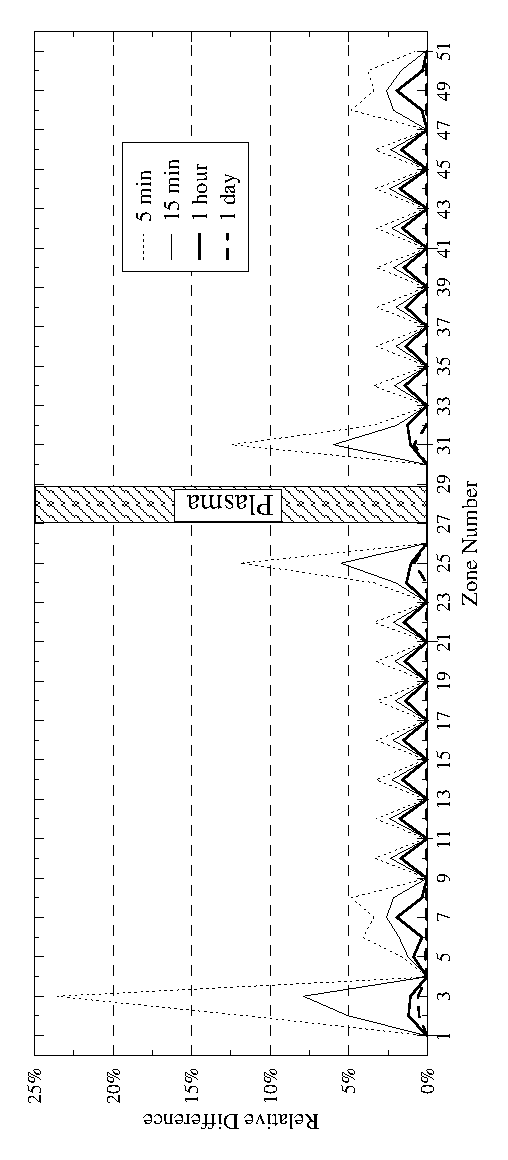
\epsfig{file=eps/ss_approx_final.eps,height=\textwidth,angle=-90}
        \caption{Relative difference between exact pulsed solution and steady state approximation at various cooling times.}
        \label{fig:rel.diff.approx}
      \end{center}
    \end{figure}
    
    The two materials with largest discrepancies are the glass
    insulator (zone \#3) and the first wall heat sink (Cu-Be-Ni in
    zones \#25 and \#31).  In the former, the activity of $^{28}$Al
    (t$_{1/2}$ = 2.25 m), responsible for over 25\% of the activity at
    a cooling time of 1 minute, is under-calculated in the
    steady-state approximation by 50\%.  The same is true of $^{66}$Cu
    (t$_{1/2}$ = 5.10 m), responsible for just under 10\% of the
    activity in the first wall.
    
  \end{section}

  \begin{section}{Advanced Features}
  
    It is not possible to validate \ALARA's complex schedule modeling
    or reverse calculation mode through comparison to other codes
    because these features are unique to \ALARA.  It is possible to
    reformulate these benchmark problems into test problems for
    \ALARA's advanced features, comparing the results to those for the
    standard benchmark problem.

    \begin{subsection}{Complex Schedule Modeling}
    
      With the standard single pulsing history capabilities validated
      against DKR in section \ref{sec:valid.pulse}, it is possible to
      construct a number of complex pulsing schedules, each reducible
      to the same pulsing schedule as the IAEA Benchmark problem.
      Four such reformulations, with increasing complexities, have
      been tested and compared to the normal pulsing problem's
      results.
    
      The first formulation splits the 94500 pulses into two groups of
      47250 pulses, and a delay of 1200 s after the first group of
      pulses.  The next formulation uses four groups of pulses of
      23625 pulses with 1200 s delay after each of the first 3 groups.
      The third formulation increases the number of levels in the
      schedule hierarchy.  The top level schedule has two
      sub-schedules.  Each sub-schedule is repeated 100 times, with
      1200 s delay after the first sub-schedule.  The first
      sub-schedule has two pulsing groups, each with 250 pulses and
      separated by a 1200 s delay.  The second sub-schedule has two
      groups of pulses with 225 and 220 pulses respectively.  The
      total number of pulses is again $\left[ 100 \times ( 250 + 250)
        + 100 \times (225 + 220) \right] = 94500$.  The last
      formulation is the most complicated.  The top level schedule
      again has two sub-schedules.  The first sub-schedule is repeated
      10 times and consists of a block of 2500 pulses followed by a
      1200 s delay and then another sub-schedule, consisting, in turn,
      of two blocks of 125 pulses, and is repeated 10 times.  The
      second sub-schedule is repeated 100 times and has one block of
      445 pulses.  Summing the entire schedule gives $\left[ 10 \times
        ( 2500 + 10 \times (125 + 125)) + 100 \times 445\right] =
      94500$ pulses.
    
      After the complete solution of all four problems, the only
      difference amongst the results was the length of time taken to
      calculate them (using the unix program 'diff' on both the output
      files and tree files showed no difference).  This is logical
      since increasing the schedule complexity increases both
      the number of matrices created and the number of matrix
      calculations required to combine their effects into the whole
      schedule.
      
    \end{subsection}
    
    \begin{subsection}{Reverse Calculation}
    
      In order to test the reverse calculation mode, it is sufficient
      to formulate a problem targeting isotopes known to be created by
      the forward calculation.  Since steel is the most prevalent
      material in the IAEA Benchmark, the 4 most significant (in terms
      of specific activity) isotopes were chosen as targets in the
      steel mixtures: $^{51}$Cr, $^{54}$Mn, $^{55}$Fe, and $^{57}$Co.
      With the goal being to determine the production of these
      isotopes from steel, all zones without stainless steel 316 were
      changed to ``void'' to reduce the computational time.
      
      The shutdown inventories for these four isotopes were identical
      to those of the forward calculation and table
      \ref{tab:valid.reverse} shows the source of each target isotope.

      \begin{table}[htbp]
        \begin{center}
          \leavevmode
          \begin{tabular}{|c|c|c|c|c|}
            \hline
            \textbf{Source}  & \multicolumn{4}{c|}{\textbf{Target isotopes}} \\\cline{2-5}
            \textbf{isotope} & $^{51}$Cr & $^{54}$Mn & $^{55}$Fe & $^{57}$Co \\\hline\hline
            $^{51}$V & 1.9 appm &  -- &  -- &  -- \\\hline
            $^{50}$Cr & 69\% & -- &  -- &  -- \\\hline
            $^{52}$Cr & 29\% & -- &  -- &  -- \\\hline
            $^{53}$Cr & 221 appm & -- &  -- &  -- \\\hline
            $^{54}$Cr & -- & 101 appm &  -- &  -- \\\hline
            $^{55}$Mn & -- & 31\% & 830 appm &  -- \\\hline
            $^{54}$Fe & 2.6\%  & 68\% & 24\% &  -- \\\hline
            $^{56}$Fe & -- & 0.65\%  & 72\%  &  -- \\\hline
            $^{58}$Ni & -- & 238 appm & 3.9\% &  100\%\\\hline
          \end{tabular}
          \caption{Sources of primary radioactive isotopes in stainless steel first wall layer.}
          \label{tab:valid.reverse}
        \end{center}
      \end{table}
      
    \end{subsection}
  \end{section}
  
  \begin{section}{Computing Resources}
    
    
    For the steady-state and pulsing code comparison, all three codes
    were used on the same IBM RS/6000 Model 595 P2SC workstation.  The
    full steady-state problem was solved by \ALARA\ in 3425 s
    (57$^m$5$^s$) and by DKR in 5253 s (1$^h$27$^m$33$^s$).  The same
    problem required 20715 s (5$^h$36$^m$25$^s$) for a previously
    developed shell-script system sequentially running FISPACT-97 for
    each of the intervals.  The pulsed problem was solved by \ALARA\ 
    in 5736 s (1$^h$35$^m$36$^s$), with 44591 nodes and a longest
    chain of 14.  DKR needed 10855 s (3$^h$0$^m$55$^s$).  FISPACT-97
    was unable to solve the pulsed problem.
    
    For the steady state problem, \ALARA\ requires a maximum of 35 MB
    of RAM and, other than the binary library of just over 11 MB, uses
    no hard drive space.  DKR required as much as 107 MB of RAM and up
    to 250 MB of temporary hard drive space in addition to its 10 MB
    text library.  Other than the 38 MB data libraries, FISPACT-97
    uses negligible quantities of RAM and hard drive space since it
    solves each interval sequentially.
    
    For the advanced feature validation, a complete set of problems
    was run on the development platform, an Intel P166MMX based
    machine running the Linux 2.0.30 operating systme.  Table
    \ref{tab:valid.runtime} shows the time required for each problem.

    \begin{table}[htbp]
      \begin{center}
        \leavevmode
        \begin{tabular}{|l|c|}
          \hline
          steady state & 17.5 m\\\hline
          basic pulsing & 24.7 m\\\hline\hline
          complex pulsing 1 & 40.3 m\\\hline
          complex pulsing 2 & 68.8 m\\\hline
          complex pulsing 3 & 70.2 m\\\hline
          complex pulsing 4 & 74.1 m \\\hline
          reverse problem & 1.7 m\\\hline
        \end{tabular}
        \caption{Runtimes for benchmark suite.}
        \label{tab:valid.runtime}
      \end{center}
    \end{table}

  \end{section}
  
  \begin{section}{Conclusions}
    
    The \ALARA\ activation code has been validated for use in
    calculating the activation of fusion power systems.  The results
    for a steady state activation problem have been compared to the
    results from two standard codes whose accuracy has been well
    documented: FISPACT-97 and DKR.  Discrepancies between the total
    activities calculated by \ALARA\ and the other codes are always
    less than 2.5\%, except where DKR is unable to calculate the
    tritium production from emitted light ions.  The results of a
    pulsing problem have been compared to DKR (FISPACT-97 was unable
    to perform such a calculation in a reasonable time).  The
    discrepancies in this case are once again primarily due to the
    lack of tritium production in DKR, and are otherwise less than
    1\%.
    
    Based on this validation and its faster and less memory-intensive
    operation, \ALARA\ is recommended for the solution of fusion
    activation problems.
    
  \end{section}

\end{chapter}

